%%%%%%%%%%%%%%%%%%%%%%%%%%%%%%%%%%%%%%%%%%%%%%%%%%%%%%%%%%%
% LaTeX Template ~ 'tau-book.tex'
% Version 2.1 (04/03/2024)
%
% Description: 
% Tau-book is a LaTeX template that offers a clean and 
% professional design for lab reports or academic papers.
% The clarity of the code structure makes it easy to 
% understand and modify for your needs. This template uses 
% an easy-to-read font and high quality equations with "stix2".
%
% Author: 
% Guillermo Jimenez (memo.notess1@gmail.com)
% 
% License:
% Creative Commons CC BY 4.0
%%%%%%%%%%%%%%%%%%%%%%%%%%%%%%%%%%%%%%%%%%%%%%%%%%%%%%%%%%%
% You may modify 'tau-book.cls' file according to your
% needs and preferences. This LaTeX class file defines 
% the document layout, formatting, and behavior.
%%%%%%%%%%%%%%%%%%%%%%%%%%%%%%%%%%%%%%%%%%%%%%%%%%%%%%%%%%%
%     BIBLIOGRAPHY WITH BIBLATEX IN EXTERNAL EDITORS:
% If the bibliography does not show up, try running the 
% 'tau-book.cls' and 'tau.bib' file with biber from the 
% MikTeX console or your preferred LaTeX distribution to 
% generate the .aux files and (re)run tau-book.tex again.
%%%%%%%%%%%%%%%%%%%%%%%%%%%%%%%%%%%%%%%%%%%%%%%%%%%%%%%%%%%
%                          WARNING:
% It is important to proceed with caution and ensure that 
% any modifications made are compatible with LaTeX 
% syntax and conventions to avoid errors or unexpected 
% behavior in the document compilation process.
%%%%%%%%%%%%%%%%%%%%%%%%%%%%%%%%%%%%%%%%%%%%%%%%%%%%%%%%%%%

\documentclass[10pt,a4paper,twoside]{tau-book}
\usepackage[english]{babel}
\usepackage{tau}
% Bibliography already loaded in tau-book.cls

%----------------------------------------------------------
% Title
%----------------------------------------------------------

\title{Medical Imaging Visualization Lab Report}

%----------------------------------------------------------
% Authors, affiliations and professor
%----------------------------------------------------------

\author[1]{Carles Matoses Gimenez}

%----------------------------------------------------------

\affil[1]{Universitat Politècnica de Catalunya - BarcelonaTech}

\professor{Imanol Munoz-Pandiella}

%----------------------------------------------------------
% Footpage notes
%----------------------------------------------------------

\institution{UPC}
\ftitle{SV}
\theday{\today} % \today
\etal{Carles Matoses Gimenez}
\course{Scientific Visualization}

%----------------------------------------------------------
% Abstract
%----------------------------------------------------------

\theabstract{This report contains information about the real time volumentric rendering shader. It explains how DVR works with the ray marching algorithm and front to back compositing. It also explains the different techniques used to improve the quality of the rendering, such as lighting, transfer functions and optimizations like empty space skipping and early ray termination. Finally, it shows some results and conclusions about the implementation.}

%----------------------------------------------------------

\keywords{\LaTeX\ class, lab report, academic paper, tau-book class, volumetric rendering.}

%----------------------------------------------------------

\begin{document}
	
    \maketitle
    \abscontent
    % \tableofcontents  % Uncomment to activate the table of contents
    \thispagestyle{firststyle}

%----------------------------------------------------------
% The document begins
%----------------------------------------------------------




\section{Introduction}

    \taustart{I}n this lab report, we present the implementation of a real-time volume rendering shader using Direct Volume Rendering (DVR) techniques. The shader is designed to visualize 3D volumetric data by employing ray marching and front-to-back compositing methods. Additionally, we incorporate fresnel effect to enhance certain visual aspects of the rendering.

\section{Rendering}
% Subjects i want to mention
% - [X] Ray-box intersection
% - emission-absorption intergrator.
%   - Front to back compositing
%   - Premultiplied alpha
%   - early ray termination
% - [X] Sampling step +  Nyquist-Shannon theorem 
% - [X] Transfer functions
% - Stable and numerically correct opacity/color accumulation
% - [X] Gradient computation for lighting
% - imatges explicant step size independent opacity

We are provided a \textbf{.raw file containing a row} (or column) \textbf{of scalars}. The name of the file contains the dimensions of the volume. We create a \textbf{3D texture in webGL} to sample the volume data. The vertex shader will recieve the vertices, normals and texture of a cube as input. For convenience, we will output the vertex position in world space. In the fragment shader, we will recieve the 3D texture, light attributes, positions in world space and TF parameters as uniforms.

\lstinputlisting[caption=Pseudocode for DVR, label={lst:listing-tex}, language=C++]{DVR_pseudocode.txt}

The Direct Volume Rendering could be done in view space to avoid some computations, but \textbf{we will do it in world space} for clarity. 
We start by computing the ray direction from the camera position to the fragment position \ref{ray-incident}. 



\textbf{We assume volume of size -1 to 1 in all axis}, this can be extended in the future to support arbitrary axis-aligned bounding boxes. The problem is that we do not have any way to know the phisical dimensions of the object before it was captured. The best guess would be to assume it was sampled with the same step size in all axis, but this is not always true. 

\begin{equation}
    \vec{r}_i = \vec{c} - \vec{f}
    \label{ray-incident}
\end{equation}

\subsection{Ray-Box Intersection}
The ray-box intersection is \textbf{computed using the slab method \texttt{intersect\_box(origin, direction)}}. For each axis, we compute the minimum and maximum intersection distances $t_{a}^{\min}$ and $t_{a}^{\max}$ using the parametric equation of the ray. Then , we compute $t_{1,a}$ and $t_{2,a}$ as the minimum and maximum of $t_{a}^{\min}$ and $t_{a}^{\max}$. Finally, we compute the near and far intersection distances $t_{\text{near}}$ and $t_{\text{far}}$ as the maximum of $t_{1,a}$ and the minimum of $t_{2,a}$ respectively. If $t_{\text{near}}$ is greater than $t_{\text{far}}$, there is no intersection. 

\subsection{Sampling Step}
For the sampling step, we use \texttt{step\_size(vec3 ray\_direction, vec3 dimensions)} that calculates the step size based on the segment we are traversing. The volume is not required to have same voxel size in all axis, we dinamically \textbf{calculate the step size for each ray individually based on the ray direction and the volume dimensions}. This method is meant to optimize ray marching to the minimum required steps at any view direction. We use the \textbf{Nyquist-Shannon \cite{5055024} theorem to avoid aliasing}, so we set the step size to half of the minimum distance between voxel centers along the ray direction. This is not done in the function for reutilization purposes.

\subsection{Transfer Function}
The \textbf{transfer function} \texttt{transfer\_function\_sigma(float density, float step\_size)} maps the density value to opacity. Color will be implemented in the lighting function. The TF \textbf{works as a rectangular window function (also Tukey window)}, where values below a minimum density are fully transparent and values above a maximum density are fully opaque. We add two more controlers to create a smooth transition between the minimum and maximum density values. The implementation is \textbf{done with conditionals} to detect the different zones and apply the corresponding formula.

\subsection{Beer-Lambert law implementaiton}
\textbf{Step size opacity independence is archieved with Beer-Lambert law \cite{mayerhofer2020bouguer}} $T=e^{-\sigma \cdot d}$ where $T$ is transmittance, $\sigma$ is extinction coefficient and $d$ is distance (step size). Sigma is $\sigma = uTFOpacity * (1.0/d)$, the $d$ terms cancel out. The opacity becomes independent of step size and only depends on uTFOpacity.

\begin{figure}[htbp]
    \centering
    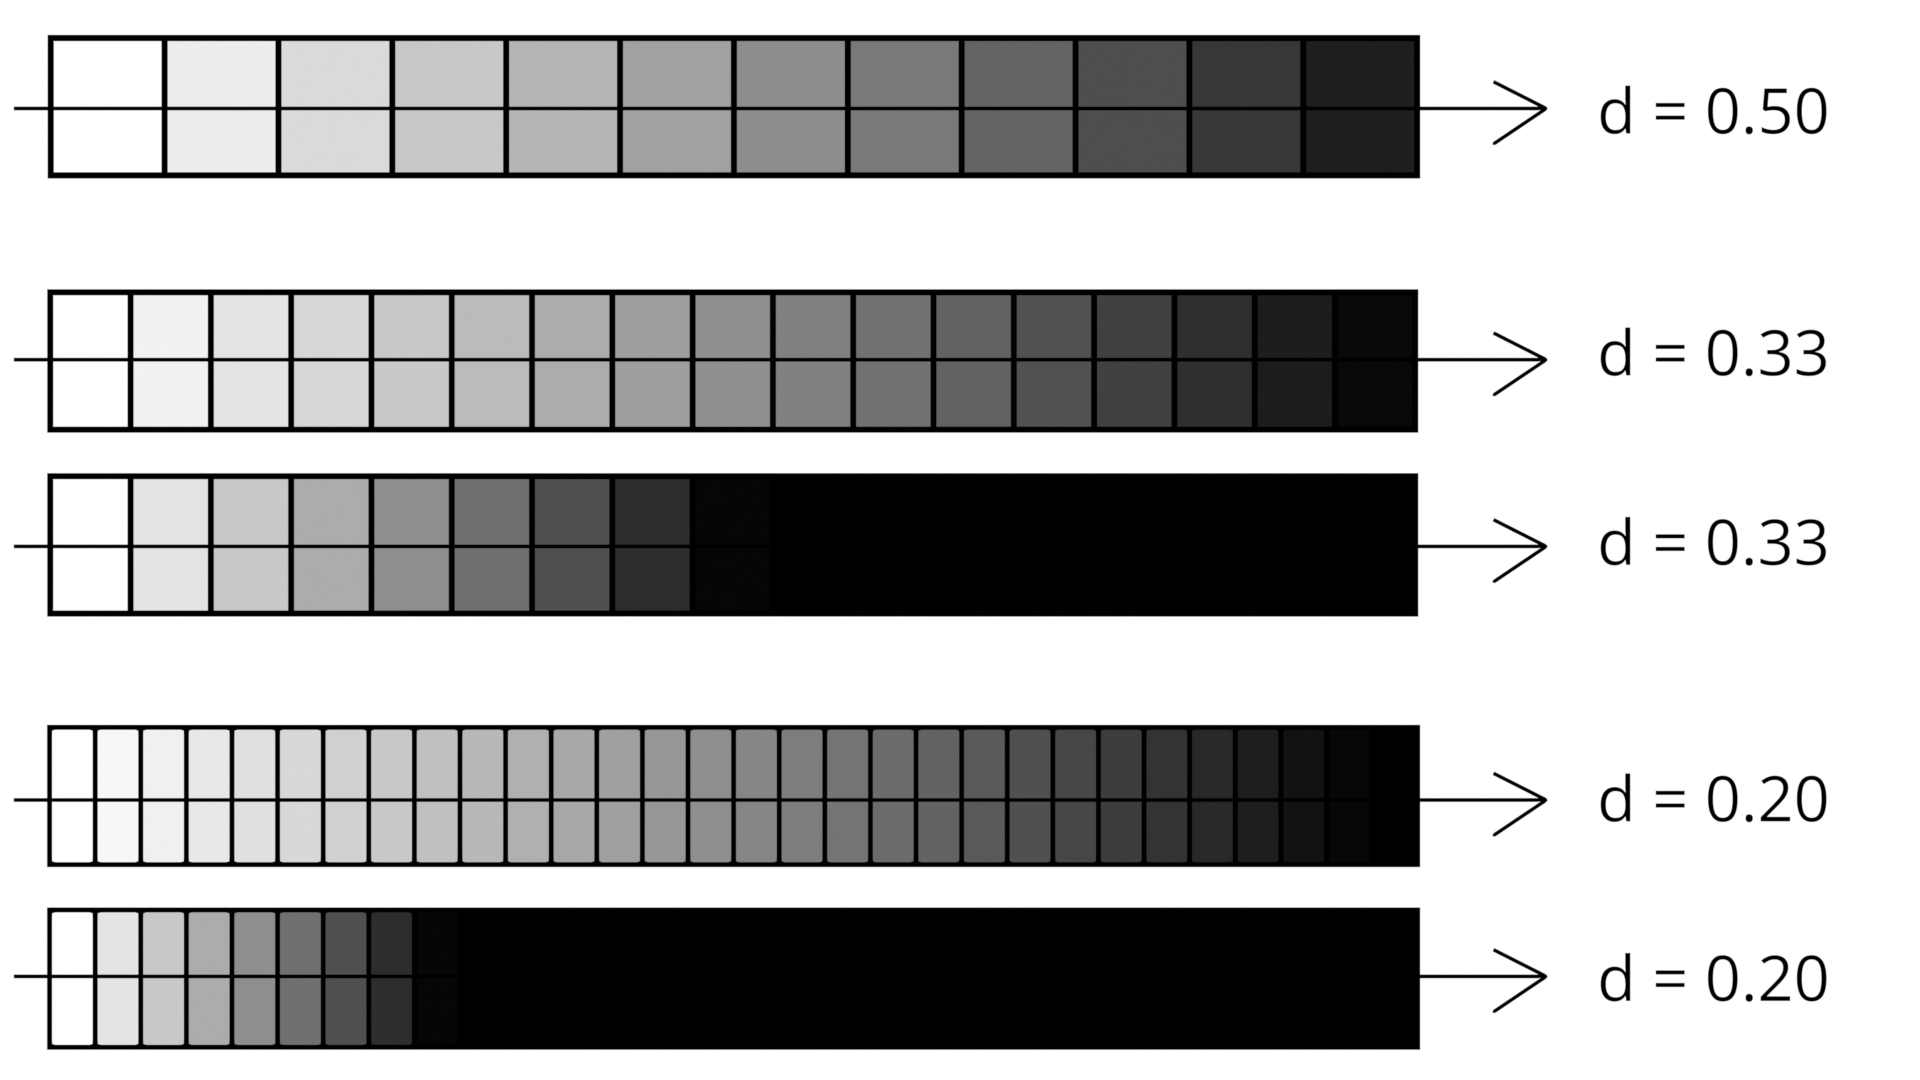
\includegraphics[width=\columnwidth]{Figures/normalized-step.png}
    \caption{Visualization showing step size independence using Beer-Lambert law normalization. If step size is not taken into account, we darken the volume faster than expected when using smaller step sizes, leading to inconsistent rendering results.}
    \label{fig:normalized-step}
\end{figure}
 
\subsection{Light Position}

We assume scene has a unique light source. Additionally, light intensity does not diminish with distance for simplicity. The light position is provided as a uniform variable to the fragment shader. For soft shadows (minimum of two light sources), we \textbf{generate points in a disc} from which we will calculate the light contribution. The disc is generated in the plane \textbf{orthogonal to the light-to-fragment direction}, with a radius controlled by the UI. This method simulates an area light source, producing softer shadows by averaging the contributions from multiple sample points on the disc.

\subsection{Color Accumulation}

Color accumulation is performed in \texttt{accumulate\_color\_and\_opacity(vec3 p\_in, vec3 p\_out, float step\_size)} using front-to-back ray marching. The \textbf{ray is sampled uniformly from the near intersection point $p_{\text{in}}$ to the far intersection point $p_{\text{out}}$.} At each step, the volume density is converted to an extinction coefficient $\sigma$ via the transfer function.

\textbf{Opacity is computed using the Beer-Lambert law over the current step length $d$}:

\begin{equation}
\alpha = 1 - \exp(-\sigma \cdot d)
\end{equation}

If the sample opacity exceeds a small threshold, \textbf{gradients are evaluated to estimate the local normal, and Phong lighting} \cite{phong1975illumination} is applied using \texttt{computeLighting}. The lighting model combines ambient, diffuse, and specular terms:
\begin{equation}
\mathbf{C}_{\text{sample}} =
\mathbf{C}_{\text{ambient}} +
\mathbf{C}_{\text{diffuse}} +
\mathbf{C}_{\text{specular}}
\end{equation}

with standard Phong definitions for each component. The shininess parameter $\alpha$ is controlled through the UI (light radius).

To account for light absorption between the current sample position and the light source, the \textbf{shaded color is multiplied by a transmittance term computed along the shadow ray using \texttt{accumulate\_opacity}}. This secondary ray march calculates the step size based on the light direction. For optimization reasons we do not reduce the step size by half when calculating shadows (becomes unnecessary expensive for non noticeable improvements).

Color and opacity are accumulated using \textbf{premultiplied alpha compositing in a front-to-back manner like in \cite{10.1145/78964.78965} and \cite{levoy1988display}:}
\begin{align}
\mathbf{C}_{\text{acc}} &\leftarrow
\mathbf{C}_{\text{acc}} + (1 - \alpha_{\text{acc}})
\cdot (\mathbf{C}_{\text{sample}} \cdot \alpha) \\
\alpha_{\text{acc}} &\leftarrow
\alpha_{\text{acc}} + (1 - \alpha_{\text{acc}}) \cdot \alpha
\end{align}

This formulation corresponds to a Riemann sum approximation of the volume rendering integral and matches the Beer-Lambert extinction model used in the implementation.

For efficiency, \textbf{early ray termination} is applied: once the accumulated opacity exceeds a threshold (e.g.\ $\alpha_{\text{acc}} > 0.95$), the ray marching loop is terminated since further contributions become negligible.

% todo show images where we dont use step size independent opacity and the artifacts that appear

\subsection{Gradient Computation}
We have tried \textbf{two methods to compute the gradients} \ref{fig:gradient}, both with advantages and disadvantages. The \textbf{first method uses density values}. This means we do not take the TFs into account. This is perfect for voxels in the margins so they \textbf{can show normals even if the TF returns maximum opacity in a rectangular window}. This gives the best results for most cases. \textbf{Hollow objects will have inverted normals if looked from the inside}. If TF removes bones and mussels to only leave skin, we will not be able to to illuminate it with the current diffuse lightning since normal directions will point outwards as expected. The \textbf{second approach is to use opacity values} from the TF. We solve the iluminaiton of hole objects but \textbf{we loose density information} when calculating the gradient.

\begin{figure}[htbp]
    \centering
    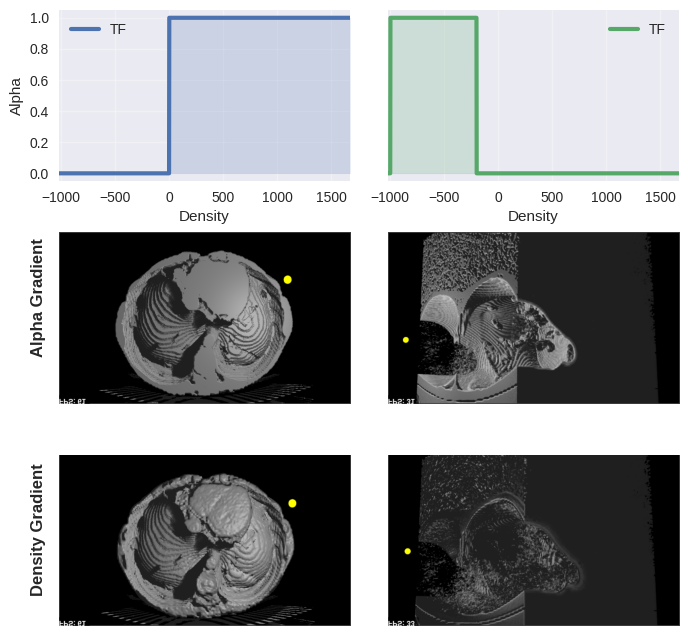
\includegraphics[width=\columnwidth]{Figures/gradient.png}
    \caption{Comparison of normals computed with opacity (left) and density (right). Notice how the opacity normals fail to capture the surface details due to the transfer function removing important density information. Density normals fail to provide correct illumination for hollow objects when viewed from the inside (normals are inverted).}
    \label{fig:gradient}
\end{figure}

The gradient $\nabla f$ at point $\mathbf{p}$ is \textbf{computed using central differences}. We sample the volume at six neighboring points displaced by $\Delta s \cdot c_{\text{smooth}}$, where $\Delta s$ is half the step size and $c_{\text{smooth}}$ is a smoothing coefficient:

\begin{align}
    \mathbf{p}_l &= \mathbf{p} + (-\Delta s \cdot  c_{\text{smooth}}, 0, 0) \\
    \mathbf{p}_r &= \mathbf{p} + (\Delta s \cdot c_{\text{smooth}}, 0, 0) \\
    \mathbf{p}_b &= \mathbf{p} + (0, -\Delta s \cdot c_{\text{smooth}}, 0) \\
    \mathbf{p}_t &= \mathbf{p} + (0, \Delta s \cdot c_{\text{smooth}}, 0) \\
    \mathbf{p}_{\text{close}} &= \mathbf{p} + (0, 0, -\Delta s \cdot c_{\text{smooth}}) \\
    \mathbf{p}_{\text{far}} &= \mathbf{p} + (0, 0, \Delta s \cdot c_{\text{smooth}})
\end{align}

The gradient is then computed as:

\begin{equation}
    \nabla f(\mathbf{p}) = \begin{pmatrix}
        f(\mathbf{p}_r) - f(\mathbf{p}_l) \\
        f(\mathbf{p}_t) - f(\mathbf{p}_b) \\
        f(\mathbf{p}_{\text{far}}) - f(\mathbf{p}_{\text{close}})
    \end{pmatrix}
\end{equation}

where $f(\mathbf{p})$ represents the sampled density (or opacity) value at position $\mathbf{p}$. The gradient vector points in the direction of maximum density increase. For surface normals, we negate this vector to obtain the outward-pointing normal: $\mathbf{n} = -\frac{\nabla f(\mathbf{p})}{|\nabla f(\mathbf{p})|}$.



Additional problems to normal calculations: \textbf{If using  density, we need to know the minimum posible value} of density since "void" will take that value (or smaller) for sampling out of the volume points. If done correctly, the model should have values between 0 and infinity but this is not the case in the medical images used in the warmup (from -1024 to 1637).
% Normals are calculated in two steps: first we compute the gradient from the density of each voxel (not opacity) which points toward maximum increase of density, then invert it to get the normal that points outside the surface. We incorrectly called this funciton \texttt{calculateNormal(vec3 point)}. We do not use alpha value for the gradient to avoid unnecessary computations. This may lead to a little more incorrect normals on rectangular window functions but it is not noticeable because of the nature of the TF where we are cutting on  density changes. This means that sampling voxel s, near voxels with lower density translated to 0 alpha will have the same effect on the gradient as if we used alpha values. The inconvinient happens when rectangular window functions only render the lower density parts of the volume, gradient will still point toward higher density values that are not rendered.  



\section{Silhouette}
% - intention: Highlight dense parts of the volume
% - Fresnel mathematical model
% - Implementation details
% - show render results on two datasets
Using the Fresnel effect, we can \textbf{highlight the silhouette of dense parts} of the volume. The classical Schlick approximation is

\begin{equation}
F(\theta) = F_0 + (1 - F_0)(1 - \cos\theta)^u
\end{equation}

where $F_0$ is the base reflectance at normal incidence, $\theta$ is the angle between the view direction and the surface normal and $u$ controls the rim sharpness. In our implementation we drop $F_0$ (set to 0) and use a simplified rim term driven by the view-normal cosine:

\begin{equation}
	ext{rim} = \bigl(1 - |\mathbf{v} \cdot \mathbf{n}|\bigr)^{p}, \qquad p = 6.0
\end{equation}

To keep the effect only on semi-opaque regions \textbf{we gate it with the accumulated opacity using a smoothstep mask}: $w = \text{smoothstep}(0.3,\,0.7,\,\alpha)\,\text{rim}$. This emphasizes edges (grazing angles) while avoiding over-brightening fully transparent or fully opaque areas \ref{fig:fresnel-function}. Figure~\ref{fig:highlightDensity} shows the effect, and Fig.~\ref{fig:smooth-function} illustrates the masking window.

\begin{figure}[htbp]
    \centering
    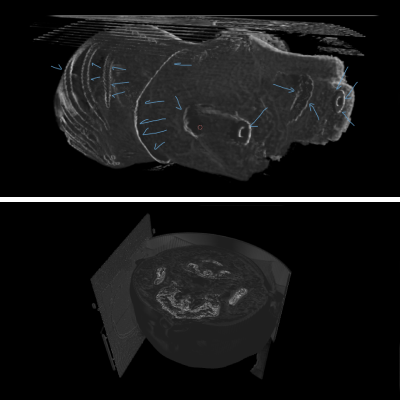
\includegraphics[width=\columnwidth]{Figures/highlightDense3.png}
    \caption{Silhouette highlighting using the Fresnel effect to emphasize dense regions of the volume. Rendered with a single light behind the model.}
    \label{fig:highlightDensity}
\end{figure}

\begin{figure}
    \centering
    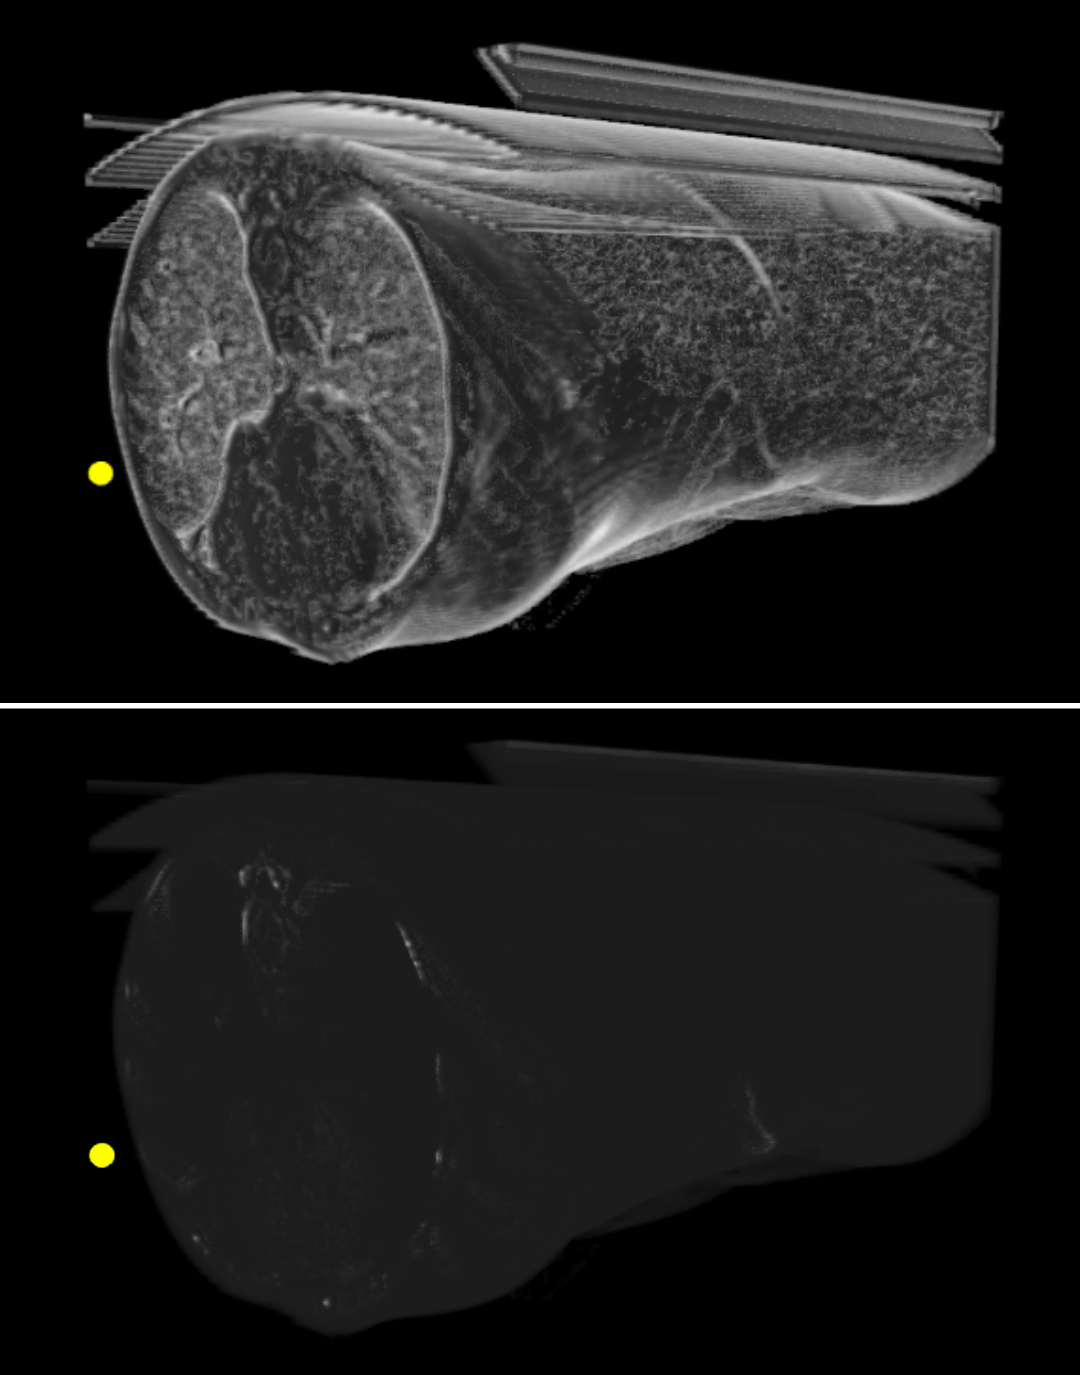
\includegraphics[width=\columnwidth]{Figures/invasiveFresnel3.png}
    \caption{Comparison of volume rendering with and without smoothstep masking of the Fresnel effect. The top image shows excessive brightening in non-dense areas without masking, while the bottom image uses smoothstep to limit the effect to highly dense regions, resulting in a more visually appealing highlight.}
    \label{fig:highlightDensity-comparison}
\end{figure}

\begin{figure}[htbp]
    \centering
    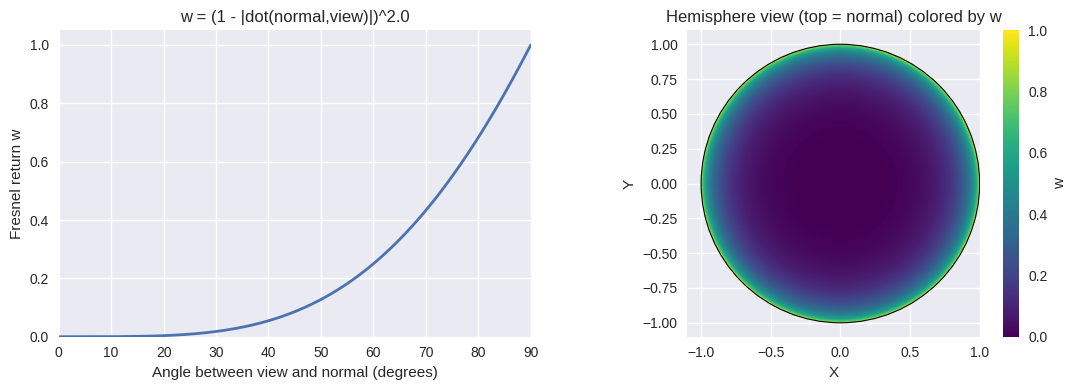
\includegraphics[width=\columnwidth]{Figures/fresnelFunction2.png}
    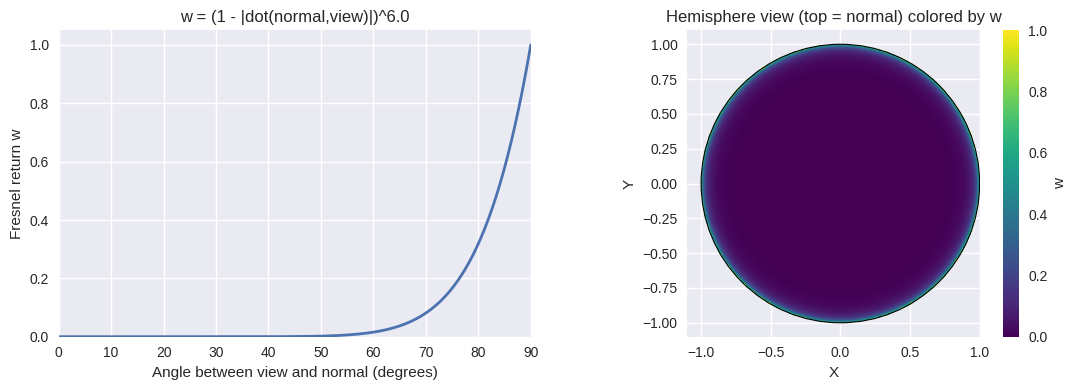
\includegraphics[width=\columnwidth]{Figures/fresnelFunction.png}
    \caption{Fresnel function showing the relationship between viewing angle and edge intensity.}
    \label{fig:fresnel-function}
\end{figure}

\begin{figure}[htbp]
    \centering
    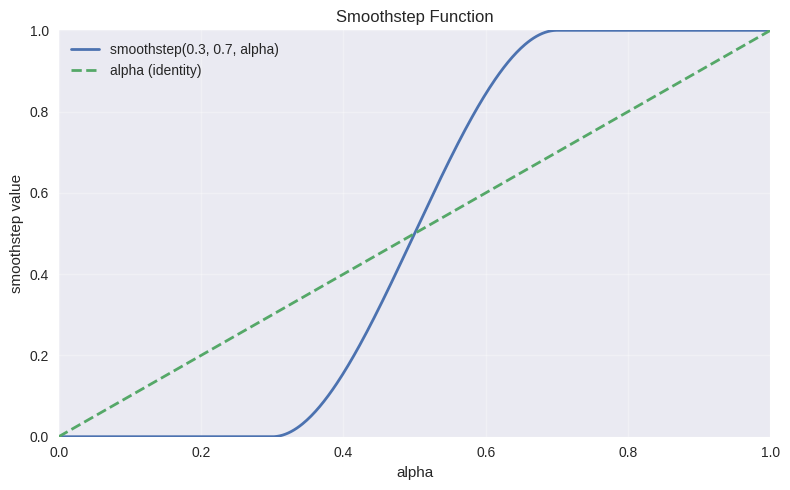
\includegraphics[width=0.5\columnwidth]{Figures/smoothfunction.png}
    \caption{Smoothstep function used to limit the Fresnel effect to specific opacity ranges.}
    \label{fig:smooth-function}
\end{figure}

\section{Performance}


% I will talk about how gpus create warps. each warp can compute 32 fragments in parallel. a gpu like gtx3080 has around 8704 cores. so 8704/32 = 272 warps can be computed in parallel. An image has 1920*1080 = 2073600 pixels. so 2073600/272 = 7617 warps are needed to compute the whole image. each warp takes multiple cycles to compute the whole raymarching. The importance of early ray termination and empty space skipping is to free warps as soon as possible to compute more warps in the same time. If a warp takes too long, the gpu will be underutilized.
\subsection{GPU usage and limitations}
GPUs achieve high parallelism by organizing threads into groups called warps, with \textbf{each warp typically consisting of 32 threads} that execute instructions simultaneously. For example, an NVIDIA RTX 3080 features 8704 CUDA cores, allowing up to 272 warps to run in parallel ($8704/32 = 272$). When rendering a 1920×1080 image (2,073,600 pixels), \textbf{approximately 7617 warps are required to process all fragments} ($2,073,600/272 \approx 7617$). Since each warp may need multiple cycles to complete complex tasks like ray marching, efficient utilization depends on freeing warps quickly. Techniques such as early ray termination and empty space skipping help release warps sooner, enabling the GPU to process more fragments in parallel and avoid underutilization caused by long-running warps.

It is necessary to understand that a \textbf{warp will not finish untill all its threads have finished}. This means that \textbf{if one thread takes a long time to compute, the whole warp will be delayed}. This is why we set a maximum number of steps for the ray marching. Another problem we percieved even though it is not too important for this project is that making a war try to \textbf{access memory in non-coalesced way will make it take much longer to fetch the data}. This happened when calculating the gradient with a large smoothing factor, since each thread in the warp was trying to access different parts of the texture memory. 

% TODO add some data to prove the performance improvements
\subsection{Early termination}
As mentioned before, we implement ... early termination techniques to improve performance:
\begin{itemize}
    \item \textbf{Opacity thresholding}: In the camera ray or the fragment-to-light rays, if the accumulated opacity exceeds a certain threshold (e.g., 0.95), we terminate the ray marching early since further contributions will be negligible. \textbf{This is the most effective optimization.}
    \item \textbf{Maximum step limit}: In some cases, we can run into scenarios where rays traverse large empty spaces or low-density regions (mostly if i implemented something wrong). This should prevent crashes but not really optimize performance unless the volume has really high resolution. 
    \item \textbf{Empty space skipping}: If the ray is traversing outside the volume bounds, we asume the step has exited the volume and terminate the ray marching. This is usually the case when a ray does not reach maximum opacity before exiting the volume. There is an improvement in performance, mostly when we have multiple lights and each light needs to compute a shadow ray. 
\end{itemize}

\begin{table}[htbp]
    \centering
    \caption{Performance impact of early termination techniques. Each row disables one optimization to show its effect on rendering speed (measured in frames per second, FPS). Tested on volume of size 128x128x100 with adaptive step size and 4 light sources. Rendered with a GTX1060 GPU.}
    \begin{tabular}{l c}
        \hline
        \textbf{Configuration} & \textbf{FPS} \\
        \hline
        All optimizations enabled & 44 FPS \\
        Without opacity thresholding & 10 FPS \\
        Without maximum step limit & 44 FPS \\
        Without empty space skipping & 21 FPS \\
        \hline
    \end{tabular}
    \label{tab:early-termination}
\end{table}


\section{Conclusions}

% I also have to talk about how the dinamic selection of samples based on the axis resolution is not actually a good idea. Scaling alpha by the step size sounds good in theory but generates too many artifacts in practice. For some reason the normalization does not work as expected, diagonal rays through the cube increase the step size and seem to miss things. I am actually not sure of why it is not working as expected since it sounds great in my paper. The results are that just deciding a constant sampling rate based on the minimum voxel size of the volume works really well and has no artifacts but it can be a bit more costly.

While dynamically selecting the sampling step size based on the axis resolution seems theoretically optimal, in practice it introduces noticeable artifacts. Scaling the opacity by the step size should normalize the results, but diagonal rays traversing the volume often use larger steps and can miss important features, leading to inconsistent rendering. Despite the mathematical justification, the normalization does not behave as expected, especially for non-axis-aligned rays. Ultimately, using a fixed sampling rate determined by the minimum voxel size produces artifact-free images, even though it may be slightly less efficient computationally.




%----------------------------------------------------------

\bibliography{tau}

%----------------------------------------------------------

\end{document}